\chapter{Propuesta}\label{chapter:proposal}

\newcommand{\dfscaption}{\hyperref[algo:dfs]{DFS-Votos}}
\newcommand{\cyclevotescaption}{\hyperref[algo:votes-cycles]{Reasignar-Votos-en-Todos-los-Ciclos}}
\newcommand{\dfsvisitcaption}{\hyperref[algo:dfs-visit]{DFS-Votos-Visita}}
\newcommand{\initdfsvertices}{\hyperref[algo:init-dfs-vertices]{Inicializar-Propiedades-de-V\'ertices}}
\newcommand{\maxincyclecaption}{\hyperref[algo:max-in-cycle]{M\'ax-Votos-en-Ciclo}}
\newcommand{\setvotestoallincyclecaption}{\hyperref[algo:set-votes-all-in-cycle]{Reasignar-Votos-en-Ciclo}}

La propuesta consta de dos ideas fundamentales: 
\begin{enumerate}
    \item el conteo de votos mediante el algoritmo de B\'usqueda del Primero en Profundidad (DFS), y
    \item el empleo de IRV para desempatar y eligir un ganador. 
\end{enumerate} 

\section{Conteo de Votos}\label{sec:dfs-counting}
El problema se puede enfocar desde la Teor\'ia de Grafos. Los votantes pueden ser vistos como v\'ertices y los votos como arcos. Contar los votos obtenidos por cada candidato se reduce a recorrer un grafo convenientemente. En esta secci\'on se detalla ese enfoque.

Sean $V$ el conjunto de los participantes  de la elecci\'on (votantes) y $f \in V \times V$ la relaci\'on de voto, esto es, $ \langle x, y \rangle \in f $ si y s\'olo si $x$ vot\'o por $ y $.  Se asume que culmin\'o el registro de todos los votos y que s\'olo existen votos v\'alidos. Cada votante puede elegir a lo sumo a otra persona, por ende, $f$ es funci\'on.

Sea $G' = \langle V, f \rangle$ el digrafo de votaci\'on, con v\'ertices en $V$ y arcos en $f$. Ahora bien, sea $G = \langle V, f^{-1} \rangle$ el digrafo que resulta de invertir los arcos de $G'$. Este \'ultimo grafo expresa la dependencia que existe entre el c\'alculo de los distintos valores de $\#_{votos}$. En efecto, si $\langle y, x \rangle \in E(G)$, entonces $\#_{votos}(y)$ depende de $\#_{votos}(x)$ para poder calcularse. Es por ello que se propone calcular los valores de $\#_{votos}$ mediante un recorrido DFS sobre $G$. 

Se propone tambi\'en considerar de manera especial a los candidatos involucrados en ciclos de votaci\'on. Estos ciclos son detectados y registrados en el recorrido DFS. Por cada ciclo, se calcula el mayor n\'umero de votos obtenidos por un v\'ertice de \'el y se le asigna esa cantidad a los restantes v\'ertices del propio ciclo. Los votantes de un mismo ciclo conf\'ian indirectamente entre ellos dos a dos, por ende, se considera justo que cada uno de ellos obtenga la misma cantidad de votos, y que esta sea la mayor obtenida por un miembro del ciclo.

\todo[inline]{@NOTE cada vez q digas algo q lleve demostracio'n, pon una referencia al lema/teorema q lo respalda en la subseccio'n d correctitud}

Los algoritmos~\ref{algo:dfs}~y~\ref{algo:dfs-visit}  constituyen adaptaciones   de las funciones DFS y DFS-Visit de \cite{intro-to-algo-3}, respectivamente. En $B$ se almacenan los arcos de retroceso de $G$.    Una vez el algoritmo~\ref{algo:dfs} termine, en $u.votos$ se tiene la cantidad de votos obtenidos por el votante representado por el v\'ertice $u$. 

\begin{algorithm}[!h]
    \caption{\dfscaption}
    \label{algo:dfs}
    \DontPrintSemicolon
    \SetAlgoLined
    \Entrada{Grafo $G = \langle V, f^{-1} \rangle$.}
    \BlankLine

    \initdfsvertices($V$)\;
    $B = \{\}$\;
    \ForEach{v\'ertice $u \in V$}{
        \If{$u.color == $ {\rm BLANCO}}{
            \dfsvisitcaption($G, u, B$)\;
        }
    }
    \cyclevotescaption($G, B$)\; \label{algo:dfs:line:votes-in-cycles}
\end{algorithm}

En \dfscaption \;primero se inicializan las propiedades de los v\'ertices. En el algoritmo~\ref{algo:init-dfs-vertices} se pueden observar esas propiedades. La propiedad $votos$ almacena la cantidad de votos recibidos por el v\'ertice. Como se puede apreciar,  \dfscaption \;difiere en muy pocos aspectos a la funci\'on DFS de \cite{intro-to-algo-3}. Uno de los m\'as significativos es el llamado a la funci\'on \cyclevotescaption \;en la l\'inea~\ref{algo:dfs:line:votes-in-cycles}. Esta funci\'on se encarga de reasignar una cantidad justa de votos a cada uno de los v\'ertices que se encuentran en un ciclo, como se mencion\'o anteriormente.  

\begin{algorithm}[!h]
    \caption{\initdfsvertices}
    \label{algo:init-dfs-vertices}
    \DontPrintSemicolon
    \SetAlgoLined
    \Entrada{Conjunto de v\'ertices $V$.}
    \BlankLine

    \ForEach{v\'ertice $u \in V$}{
        $u.color =$ BLANCO\;
        $u.votos = 0$\;
    }
\end{algorithm}

El algoritmo~\ref{algo:dfs-visit} calcula los votos obtenidos por $u$ y a\~nade a $B$ los arcos de retroceso encontrados durante el proceso. Se denota por $V_u$ al conjunto de los v\'ertices adyacentes a $u$, esto es
$$
V_u = \{ v \in V \;|\; \langle u, v \rangle \in E(G) \}.
$$

\begin{algorithm}[!h]
    \caption{\dfsvisitcaption}
    \label{algo:dfs-visit}
    \DontPrintSemicolon
    \Entrada{Grafo $G$; v\'ertice $u$; conjunto $B$ de arcos de retroceso.}     
    \BlankLine

    $u.color =$ GRIS\;

    \ForEach{$v \in V_u$}{ \label{algo:dfs-visit:line:arc-foreach}
        \If{$v.color ==$ {\rm BLANCO}}{
            \dfsvisitcaption($G, v, B$)\;\label{algo:dfs-visit:line:visit}
        }\lElse{\If{$v.color ==$ {\rm GRIS}}{
            $B = B \cup \{\langle u, v \rangle\}$\; \label{algo:dfs-visit:line:add-B}
        }}
        \If{$v.color ==$ {\rm NEGRO}}{ \label{algo:dfs-visit:line:if-black}
            $u.votos = u.votos + v.votos + 1$\; \label{algo:dfs-visit:line:votes}
        }
        \label{algo:dfs-visit:line:if-black:end}
    }
    \label{algo:dfs-visit:line:arc-foreach:end}
    $u.color =$ NEGRO\;\label{algo:dfs-visit:line:set-black}
\end{algorithm}

El ciclo de las l\'ineas~\ref{algo:dfs-visit:line:arc-foreach}-\ref{algo:dfs-visit:line:arc-foreach:end} itera por todos los arcos salientes de $u$. N\'otese que $v \in V_u$ si y s\'olo si $v$ vot\'o por $u$, por definici\'on de $G$.  Se a\~nade un nuevo arco de retroceso a $B$ en la l\'inea~\ref{algo:dfs-visit:line:add-B}. Un arco $\langle u, v \rangle$ es de retroceso si y s\'olo si $v$ es gris cuando se explora ese arco por primera vez \citep{intro-to-algo-3}. El n\'umero de votos obtenidos por $u$ es actualizado solamente en la l\'inea~\ref{algo:dfs-visit:line:votes}, cuando $v$ es negro. Esto se debe a que los votos obtenidos por $v$ se encuentran bien calculados cuando este es negro. Todos los votos obtenidos por $v$, m\'as el voto que este le confiere a $u$, son contados como votos de  $u$. N\'otese que el bloque de las l\'ineas~\ref{algo:dfs-visit:line:if-black}-\ref{algo:dfs-visit:line:if-black:end} es un ``\textbf{si}'', y no un ``\textbf{en otro caso si}''. Esto es intencional y permite que se actualicen los votos de $u$ correctamente, incluso cuando $\langle u, v \rangle$ es un arco de \'arbol de $G_\pi$. 

El algoritmo~\ref{algo:votes-cycles} considera todos los ciclos de $G$. En cada iteraci\'on, se calcula el mayor n\'umero de votos obtenidos por un v\'ertice del ciclo y se le asigna esa cantidad a los restantes v\'ertices del propio ciclo. 


\begin{algorithm}[!h]
    \caption{\cyclevotescaption}
    \label{algo:votes-cycles}
    \DontPrintSemicolon
    \SetAlgoLined
    \Entrada{Grafo $G = \langle V, f^{-1} \rangle$; conjunto $B$ de arcos de retroceso.}     
    \BlankLine

    \ForEach{$\langle u, v \rangle \in B$}{
        $m = $ \maxincyclecaption($\langle u, v \rangle, f$)\;
        \setvotestoallincyclecaption($m, \langle u, v \rangle, f$)\;
    }
\end{algorithm}

Dado un arco de retroceso $\langle u, v \rangle$ y la funci\'on de votaci\'on $f$, \maxincyclecaption \;itera por todos los v\'ertices del ciclo al que ese arco pertenece, mediante m\'ultiples aplicaciones de $f$. El algoritmo devuelve la mayor cantidad de votos obtenidos por alg\'un v\'ertice del ciclo. 

\begin{algorithm}[!h]
    \caption{\maxincyclecaption}
    \label{algo:max-in-cycle}
    \DontPrintSemicolon
    \SetAlgoLined
    \Entrada{Arco de retroceso $\langle u, v \rangle$; funci\'on de votaci\'on $f$.}     
    \Salida{Mayor n\'umero de votos obtenidos por un v\'ertice del ciclo.}
    \BlankLine

    $m = v.votos$\;\label{algo:max-in-cycle:line:m-declaration}
    $x = u$\;
    \While{$x \neq v$}{
        $m = \max(m, x.votos)$\;
        $x = f(x)$\;
    }
    \Return{$m$}\;
\end{algorithm}

El algoritmo~\ref{algo:set-votes-all-in-cycle} itera de igual manera por todos los v\'ertices del ciclo al que pertenece el arco de retroceso dado. La cantidad de votos dada ($m$) es asignada a cada v\'ertice del ciclo.

\begin{algorithm}[!h]
    \caption{\setvotestoallincyclecaption}
    \label{algo:set-votes-all-in-cycle}
    \DontPrintSemicolon
    \SetAlgoLined
    \Entrada{$m$ votos a asignar; arco de retroceso $\langle u, v \rangle$; funci\'on de votaci\'on $f$.}     
    \BlankLine

    $x = u$\;
    \While{$x \neq v$}{
        $x.votos = m$\;
        $x = f(x)$\;
    }
    $v.votos = m$\;
\end{algorithm}

Hasta aqu\'i llega la propuesta. En las secciones siguientes se demuestra  su correctitud y complejidad temporal.

\subsection{Correctitud}
Dos puntos deben ser probados para garantizar la correctitud de la propuesta:
\begin{enumerate}
    \item \label{item:dfs-votes-num} la DFS calcula correctamente los valores de $\#_{votos}$, incluso cuando $G$ posee ciclos; y
    \item \label{item:reassign-votes} a los candidatos de un mismo ciclo se les asignan la misma cantidad de votos, igual al mayor valor de $\#_{votos}$ en el ciclo. 
\end{enumerate}

El lema~\ref{lemma:dfs-visit} contribuye a la demostraci\'on del punto~\ref{item:dfs-votes-num}. En \'el se demuestra que los valores de $\#_{votos}$ son calculados correctamente cuando el grafo no posee ciclos.

\begin{lemma}\label{lemma:dfs-visit}
    Sea $B$ el conjunto de todos los arcos de retroceso. Sea el grafo $G_{DAG} = \langle V(G), E(G) - B \rangle$.  Luego de que el llamado a \dfsvisitcaption($G_{DAG}, u, B$) culmina, se cumple que $u.votos = \#_{votos}(u)$ en $G_{DAG}$.
\end{lemma}

\begin{proof}
    Como en $G_{DAG}$ no hay ciclos, entonces ning\'un v\'ertice $v$ adyacente $u$ puede ser gris cuando se visita a $u$.

    A continuaci\'on se emplea la variante fuerte del Principio de Inducci\'on Matem\'atica sobre la propiedad:
    \begin{center}
        $P(n, u)$ := el lema se cumple cuando el v\'ertice $u$ es el $n$-\'esimo en volverse negro.
    \end{center}

    N\'otese que un v\'ertice $u$ se vuelve negro si y s\'olo si se ejecuta la l\'inea \ref{algo:dfs-visit:line:set-black} del algoritmo~\ref{algo:dfs-visit} sobre $u$.

    Si $n=1$, entonces cuando se visita a $u$ ninguno de sus adyacentes es blanco o negro. Luego, no existe un arco saliente de $u$ en $G$. Esto implica que la propiedad $u.votos$ no se actualiza y mantiene su valor inicial $0$ al culminar la visita sobre $u$. Tambi\'en implica que $\#_{votos}(u) = 0$. Queda demostrado $P(1, u)$, para todo $u \in V$.

    Sea $n>1$. Sup\'ongase que $P(k, x)$ se cumple para todo $x \in V$ y $k < n$. Todo v\'ertice $v$ adyacente a $u$ cumple que es blanco o negro cuando se visita a $u$. Si es blanco, se visita en la l\'inea~\ref{algo:dfs-visit:line:visit} y al culminar la visita se vuelve negro. Luego, en cualquier caso, la l\'inea~\ref{algo:dfs-visit:line:votes} se ejecuta. $P(k_v, v)$ se cumple para alg\'un $k_v < n$, por ende, $v.votos = \#_{votos}(v)$. Al culminar la visita sobre $u$, se cumple que
    \begin{align*}
        u.votos &= \sum_{v \in V_u} (v.votos + 1) \\
        &= |V_u| + \sum_{v \in V_u} v.votos \\
        &= |V_u| + \sum_{v \in V_u} \#_{votos}(v) \\
        &= \#_{votos}(u)
    \end{align*}
\end{proof}

El lema~\ref{lemma:one-cycle-only} afirma la imposibilidad de que un v\'ertice pertenezca a dos ciclos distintos de $G'$.  Este resultado es empleado en la demostraci\'on de la correctitud de los algoritmos~\ref{algo:max-in-cycle}~y~\ref{algo:set-votes-all-in-cycle}. N\'otese que todo ciclo en $G'$ posee un ciclo an\'alogo en $G$.
\begin{lemma}\label{lemma:one-cycle-only}
    Sean $c_1$ y $c_2$ dos ciclos de $G'$. Si el v\'ertice $u$ pertenece a $c_1$ y  a $c_2$, entonces $c_1 = c_2$.
\end{lemma}

\begin{proof}
    Como $u$ pertenece a $c_1$ y $c_2$, existen dos caminos simples $p_1 = u \leadsto x$ y $p_2 = u \leadsto y$, tal que $\langle x, u \rangle, \langle y, u \rangle \in E(G')$. Como $E(G') = f$, entonces $p_1$ y $p_2$ son de la forma
    $$
    p_1 = \langle u, f(u), f(f(u)), ..., f^k(u) = x \rangle \quad \text{y} \quad p_2 = \langle u, f(u), f(f(u)), ..., f^t(u) = y \rangle
    $$
    Sin p\'erdida de generalidad, se puede asumir que $k \leq t$. Si $k < t$, entonces $k+1 \leq t$, de donde $f^{k+1}(u)$ pertenece a $p_2$. Pero como $\langle x, u \rangle \in E(G')$, entonces
    $$
    f^{k+1}(u) = f(f^k(u)) = f(x) = u.
    $$
    Esto es imposible, ya que en $p_2$ no se repiten v\'ertices. Por lo tanto, $k = t$ y $p_1 = p_2$, lo que implica que $c_1 = c_2$.
\end{proof}

El lema~\ref{lemma:cycle-iteration} prueba la correctitud de \maxincyclecaption \;y \setvotestoallincyclecaption.

\begin{lemma}\label{lemma:cycle-iteration}
    Sea $c$ el ciclo al que pertenece el arco de retroceso $\langle u, v \rangle$. Los algoritmos~\ref{algo:max-in-cycle}~y~\ref{algo:set-votes-all-in-cycle} iteran satisfactoriamente por todos los v\'ertices de $c$ y s\'olo por ellos.
\end{lemma}

\begin{proof}
    Ambos algoritmos reciben un arco de retroceso $\langle u, v \rangle$. Se cumple entonces que $u$ es un descendiente de $v$ en $G_\pi$ \citep{intro-to-algo-3}. Luego, existe un camino en $G$ desde $v$ hasta $u$. Esto significa que existe  un camino simple desde $u$ hasta $v$ en $G'$. Como $E(G') = f$, entonces ese camino es \'unico y de la forma
    $$
    \langle u, f(u), f(f(u)), ..., f^k(u) = v \rangle.
    $$
    Por ende, en $k$ iteraciones del ciclo de \maxincyclecaption \;o de \setvotestoallincyclecaption, se llega a $v$ y el ciclo se detiene. Las iteraciones fueron realizadas  por y s\'olo por los v\'ertices del ciclo de $G$ del cual $\langle u, v \rangle$ es arco de retroceso, excepto $v$. No considerar a $v$ en el ciclo obliga a ambos algoritmos a tenerlo en cuenta de manera separada.  En el caso de \maxincyclecaption, a $m$ se le asigna el valor de $v.votos$ en la l\'inea \ref{algo:max-in-cycle:line:m-declaration}. En el caso de \setvotestoallincyclecaption, se le asigna en la \'ultima l\'inea a $v.votos$ el valor de $m$. Todo esto hace que ambos algoritmos sean correctos.
\end{proof}

Finalmente, el lema~\ref{lemma:reassign-votes} prueba el punto~\ref{item:reassign-votes} de la propuesta general.

\begin{lemma}\label{lemma:reassign-votes}
    El algoritmo \cyclevotescaption \;visita dos y s\'olo dos veces a todo v\'ertice perteneciente a un ciclo de $G$. Una de esas veces es en el algoritmo~\ref{algo:max-in-cycle} y la otra es en el algoritmo~\ref{algo:set-votes-all-in-cycle}.
\end{lemma}

\begin{proof}
    Sea $x$ un v\'ertice perteneciente a un ciclo $c$ de $G$. Luego, existe un y s\'olo un arco $\langle u, v \rangle$ de retroceso que pertenece a $c$. Se cumple que $\langle u, v \rangle \in B$ y, por ende, se considera en alguna iteraci\'on del algoritmo \cyclevotescaption. Por el lema~\ref{lemma:cycle-iteration}, al invocar a \maxincyclecaption \;y \setvotestoallincyclecaption \;en $\langle u, v \rangle$, $x$ es considerado una y s\'olo una vez en cada uno. 

    Si $x$ pertenece a un ciclo de $G$, entonces tambi\'en pertenece a un ciclo  $c'$ de $G'$. Por el lema~\ref{lemma:one-cycle-only}, $x$ no pertenece a un ciclo distinto de $c'$ en $G'$. Por ende, el v\'ertice tampoco pertenece a un ciclo distinto de $c$ en $G$. Luego, $x$ es considerado s\'olo dos veces por el algoritmo~\ref{algo:votes-cycles}: una vez en el algoritmo~\ref{algo:max-in-cycle} y una segunda vez en el algoritmo~\ref{algo:set-votes-all-in-cycle}.
\end{proof}

El teorema~\ref{theorem:counting} re\'une los anteriores resultados para probar la correctitud de toda la propuesta.

\begin{theorem}\label{theorem:counting}
    El algoritmo \dfscaption \;es correcto.
\end{theorem}

\begin{proof}
    Inicialmente, todos los v\'ertices son blancos y no tienen votos. Cuando el ciclo de \dfscaption \;culmina, todo v\'ertice ha sido visitado por \dfsvisitcaption. Luego, por el lema~\ref{lemma:dfs-visit}, se cumple que $u.votos = \#_{votos}(u)$ en $G_{DAG}$, para todo $u \in V$. El grafo $G$ es el resultado de colocar en $G_{DAG}$ los arcos de $B$. Luego, el comportamiento del algoritmo~\ref{algo:dfs-visit} sobre $G_{DAG}$ es el mismo que sobre $G$, en lo que se refiere a conteo de votos. \todo{@NOTE quiza' c puede dejar ma's claro}

    Por el lema~\ref{lemma:cycle-iteration}, se cumple que los algoritmos \maxincyclecaption \;y \setvotestoallincyclecaption \;son correctos.  Por el lema~\ref{lemma:reassign-votes} y su demostraci\'on, se cumple que el algoritmo~\ref{algo:votes-cycles} itera por y s\'olo por todos los ciclos de $G$. Por todo esto, el algoritmo \cyclevotescaption \;es correcto.

    Queda demostrado que el algoritmo \dfscaption \;es correcto.
\end{proof}


\subsection{Complejidad Temporal}\label{sec:dfs-counting:time}
En esta secci\'on se asume que $G$ est\'a representado mediante listas de adyacencia y que evaluar $f$ toma $O(1)$.

Hasta el fin del ciclo de \dfscaption, el algoritmo se ejecuta en tiempo $O(b_1(|V| + |E|))$, donde $b_1$ es el costo m\'aximo de a\~nadir un arco a $B$. Como $f$ es funci\'on, entonces 
$$
O(b_1(|V| + |E|)) = O(b_1(|V| + |f|)) = O(b_1(|V| + |V|)) = O(b_1|V|).
$$

De los lemas~\ref{lemma:reassign-votes}~y~\ref{lemma:cycle-iteration} y sus respectivas demostraciones se desprende que el algoritmo \cyclevotescaption \;se ejecuta en tiempo $O(b_2|V|)$, donde $b_2$ es el m\'aximo costo de consultar el $i$-\'esimo arco de $B$, para todo $i, 1 \leq i \leq |B|$.

Por todo lo anterior, la propuesta dada para contar los votos recibidos por los candidatos se ejecuta en tiempo $O((b_1 + b_2)|V|)$. Si $B$ se implementa mediante una lista enlazada, entonces $b_1, b_2 \in O(1)$ y el algoritmo \dfscaption \;se ejecuta en tiempo $O(|V|)$.


\section{Desempate con IRV}\label{sec:irv+time-untie}
Sean $m = \max\{ u.votos \;|\; u \in V \}$ y $W = \{ u \in V \;|\; u.votos = m \}$. El ganador del proceso electoral se encuentra en $W$. Si $|W| = 1$, entonces se declara como ganador al \'unico elemento de $W$. Para determinar qui\'en gana cuando $|W| > 1$, se emplea una adaptaci\'on del m\'etodo de desempate instant\'aneo. 

De la secci\'on~\ref{sec:irv} se conoce que para utilizar ese m\'etodo es necesario definir:
\begin{enumerate}
    \item un \textit{ranking} de votaci\'on para cada votante, y
    \item una manera de seleccionar qu\'e candidato eliminar en cada ronda, en caso de que m\'as de uno  obtenga la menor cantidad de votos.
\end{enumerate}  

\subsection{\textit{Rankings}}
Un \textit{ranking} de candidatos es por definici\'on una lista de personas preferidas por un votante, en orden ascendente de preferencia. Se propone determinar la preferencia de un votante $x$ por  un candidato $y$, por la distancia de $x$ a $y$ en el \'unico camino simple que puede conectarlos en $G'$. Mientras m\'as cerca se encuentren, m\'as fuerte es la preferencia. En esta secci\'on se define formalmente la propuesta.

Sea $x \in V$ un v\'ertice cualquiera de $G'$. Sea $P(x)$ un camino simple maximal de $G'$ que comienza en $x$. Luego,
$$
P(x) = \langle x, f(x), f(f(x)), \ldots, f^{k}(x) \rangle.
$$
Como $f$ es funci\'on, entonces $P(x)$ es \'unico. 

\begin{definition}\label{def:ranking}
    El \textit{ranking} de $x$ se define como  la subsecuencia maximal de $P(x)$ de v\'ertices distintos de $x$ que est\'an en $W$. El orden en el que aparecen los votantes en el \textit{ranking} es el mismo que el orden en el que aparecen en la subsecuencia.
\end{definition}

En la figura~\ref{fig:graph-13-voters-2-cycles} se representa un grafo de votaci\'on con 13 votantes y 2 ciclos.

\begin{figure}[h!]
    \centering
    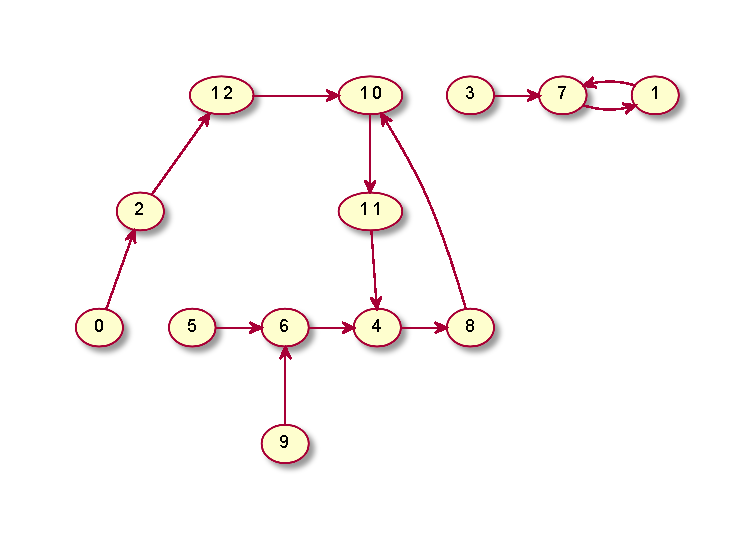
\includegraphics[scale=.9]{Graphics/graph-13-voters-2-cycles-largest-has-4.pdf}
    \caption{Grafo de votaci\'on con 13 votantes y 2 ciclos.}
    \label{fig:graph-13-voters-2-cycles}
\end{figure}
\todo[inline]{@TODO pon en amarillo a la gente q esta'n empatadas}

En ese caso, se tiene que $m = 9$ y $W = \{ 4, 8, 10, 11 \}$. En la tabla~\ref{tab:rankings-13-voters} se muestran los \textit{rankings} de cada votante.

\begin{table}[h!]
    \centering
    \begin{tabular}{|c|c|c|c|c|c|c|c|c|c|c|c|c|c|}
        \hline
        posici\'on/votante & 0  & 1  & 2  & 3  & 4  & 5  & 6  & 7  & 8  & 9  & 10 & 11 & 12 \\ \hline
        1                  & 10 &    & 10 &    & 8  & 4  & 4  &    & 10 & 4  & 11 & 4  & 10 \\ \hline
        2                  & 11 &    & 11 &    & 10 & 8  & 8  &    & 11 & 8  & 4  & 8  & 11 \\ \hline
        3                  & 4  &    & 4  &    & 11 & 10 & 10 &    & 4  & 10 & 8  & 10 & 4  \\ \hline
        4                  & 8  &    & 8  &    &    & 11 & 11 &    &    & 11 &    &    & 8  \\ \hline
    \end{tabular}
    \caption{Ejemplo de \textit{rankings} para 13 votantes (ver figura~\ref{fig:graph-13-voters-2-cycles}).}
    \label{tab:rankings-13-voters}
\end{table}

N\'otese que los \textit{rankings}  de los votantes 1, 3 y 7 est\'an vac\'ios, ya que no existe un camino en el grafo desde alguno de ellos hacia un v\'ertice de $W$.

\subsection{Eliminando por Tiempo}\label{sec:irv+time-untie:removing}
Cuando en una ronda de IRV dos o m\'as candidatos poseen la menor cantidad de votos, es preciso decidir a cu\'al de ellos eliminar. Se propone eliminar al que obtuvo esa cantidad de votos m\'as tarde en el tiempo. La propuesta se basa en la hip\'otesis de que si un candidato obtuvo sus votos en menos tiempo que otro, entonces los votantes del primero poseen m\'as seguridad y confianza en su elecci\'on que los votantes del segundo. Esta hip\'otesis se hace m\'as fuerte cuando es menos el conocimiento que poseen los votantes sobre los candidatos antes de que comience la elecci\'on. 
\todo[inline]{@TODO propo'n una manera d minimizar ese conocimiento o mira a ver si precisamente esa es una caracter\'istica del problema}

A continuaci\'on se formaliza la propuesta.


Cada voto se registra en el sistema en un tiempo determinado. Sea $t(x)$ el tiempo en el que el voto de $x$ es registrado. $t$ es funci\'on, ya que de cada persona se puede registrar a lo sumo un voto v\'alido. Esta funci\'on est\'a indefinida para las personas que no votaron.

Si antes de la primera ronda de IRV, $y$ aparece en el \textit{ranking} de $x$, entonces $y = f^r(x)$, o sea, existe una secuencia de v\'ertices $\langle x = p_1, p_2, ..., p_{r+1} = y \rangle$, tal que $p_i$ vot\'o por $p_{i+1}$, para todo $i$ con $1 \leq i \leq r$ (definici\'on~\ref{def:ranking}).  Se puede decir que $x$ vot\'o por $y$ directa (si $r=1$) o indirectamente (si $r>1$) y que $y$ obtuvo ese voto en el tiempo $\max (t(p_1), t(p_2), ..., t(p_r))$, el cual se puede denotar por $t_{rank}(x, y)$. 

Si en una ronda cualquiera de IRV, $y$ aparece en la primera posici\'on del \textit{ranking} de $x$, entonces $x$ vot\'o por $y$ directa o indirectamente. En cualquier caso, $t_{rank}(x, y)$ es una definici\'on para el tiempo en que $y$ obtiene ese voto. Sup\'ongase que $y$ se encuentra en la primera posici\'on de los \textit{rankings} de $x_1, x_2, ..., x_s$ en una ronda determinada de IRV. Luego, $y$ tiene $s$ votos en IRV y se dice que los obtuvo en tiempo 

\begin{equation}\label{eq:max-rank-time}
   t_{ronda}(y) = \underset{1 \leq i \leq s}{\max} \{ t_{rank}(x_i, y) \}. 
\end{equation}

Finalmente, de todas las personas con la menor cantidad de votos en una ronda de IRV, se propone eliminar a la que obtuvo sus votos m\'as tarde en el tiempo, esto es, la que tiene mayor valor  de $t_{ronda}$. 

En este punto puede surgir la interrogante: ?`la persona a eliminar es \'unica? La siguiente secci\'on lo aclara.

\subsubsection{Unicidad}
S\'olo existe un candidato que cumple con el criterio de eliminaci\'on en cada ronda. Esta proposici\'on es verdadera bajo la hip\'otesis de que dos candidatos no votaron al mismo tiempo. Est\'a respaldada por el corolario~\ref{corollary:irv}, el cual es una consecuencia directa del teorema~\ref{theorem:irv}.

\begin{theorem}\label{theorem:irv}
    Si $t$ es inyectiva y $t_{ronda}(y_1) = t_{ronda}(y_2)$, entonces $y_1 = y_2$.
\end{theorem}

\begin{proof}
    Sea $T = t_{ronda}(y_1)$ y sup\'ongase que $T = t_{ronda}(y_2)$. Entonces $t_{rank}(x_{i}, y_1) = t_{rank}(x_{j}, y_2) = T$ \todo{@FIXME se sale del margen}, para alg\'un $i$ y $j$, tal que $y_1$ y $y_2$ aparecen en la primera posici\'on de los \textit{rankings} de $x_{i}$ y $x_{j}$, respectivamente. Luego, en $G'$ existen los caminos
    $$
    p_1 = \langle x_{i}, f(x_i), f(f(x_i)), ..., f^k(x_i) = y_1 \rangle \quad \text{y} \quad p_2 = \langle x_{j}, f(x_j), f(f(x_j)), ..., f^l(x_j) = y_2 \rangle,
    $$
    tal que $f^\alpha(x_i)$ y $f^\beta(x_j)$ no se encuentran en los \textit{rankings} de $x_i$ y $x_j$, respectivamente, para todo $\alpha$ con $ 1 \leq \alpha < k$ y $\beta$ con $ 1 \leq \beta < l$. Si $t$ es inyectiva, como $t(f^\alpha(x_i)) = t(f^\beta(x_j)) = T$, entonces $f^\alpha(x_i) = f^\beta(x_j)$, para alg\'un $\alpha$ con $ 1 \leq \alpha < k$ y $\beta$ con $ 1 \leq \beta < l$. Sin p\'erdida de generalidad, se puede asumir que $k \leq l$. Luego, existe un subcamino de $p_2$ de la forma
    $$
        f^\beta(x_j) \leadsto f^k(x_i) \leadsto f^l(x_j).
    $$
    N\'otese que $f^k(x_i) = y_1$ y $f^l(x_j) = y_2$.  Si $k<l$, entonces $y_1$ se encuentra antes de $y_2$ en el \textit{ranking} de $x_j$ en la ronda actual, lo cual es imposible. Luego, $k=l$ y $y_1 = y_2$.
\end{proof}

\begin{corollary}\label{corollary:irv}
    Si $t$ es inyectiva, entonces no existen dos candidatos distintos con la menor cantidad de votos en una ronda de IRV, que posean el mismo valor de $t_{ronda}$.
\end{corollary}

\begin{proof}
    Inmediata del teorema~\ref{theorem:irv}.
\end{proof}

% Formalmente, el \textit{ranking} de $x$ es
% $$
% R(x) = \langle y_{i_1}, y_{i_2}, \ldots, y_{i_t} \rangle, \quad 1 \leq i_1 \leq i_2 \leq \ldots \leq i_t \leq k, \quad y_{i_j} \in W \setminus D, \; 1 \leq \forall j \leq t.
% $$
% Formalmente, el \textit{ranking} de $x$ es
% $$
% R(x) = \langle y_{i_1}, y_{i_2}, \ldots, y_{i_t} \rangle, \quad 1 \leq i_1 \leq i_2 \leq \ldots \leq i_t \leq k, \quad y_{i_j} \in W \setminus D, \; 1 \leq \forall j \leq t.
% $$

% @FIXME change blankspace between (figura|tabla|algoritmo) and (\ref|\cite) command for a ~
% @TODO remove \SetAlgoLined from all algorithms